\documentclass{article}
\usepackage{amsmath}
\usepackage{amssymb}
\usepackage{graphicx}
\usepackage{hyperref}
\usepackage[version=4]{mhchem}

\title{Problem 9}
\date{}

\begin{document}
\maketitle

\section*{Problem}
In rectangle \(A B C D\), the diagonal \(B D=25\), and \(A D / A B=3 / 4\). Suppose that \(E\) is a point on line \(B D\) such that \(C E \perp B D\). Connect \(A E\). What is the area of \(\triangle A D E\) ?\\
(A) 90\\
(B) 105\\
(C) 115\\
(D) 120\\
(E) 140\\
\centering
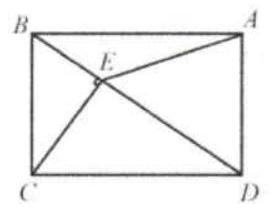
\includegraphics[width=\textwidth]{images/089(1).jpg}

\section*{Solution}
Solution not available.

\end{document}
